\section{Floss for Science: A podcast promoting open source software}

\begin{frame}{Floss for Science}
\framesubtitle{A podcast promoting open source software}

    \begin{columns}
    \column{0.5\textwidth}
    \begin{itemize}
        \item \textit{FLOSS for Science} is a podcast with the goal of showcasing free, libre and open source software uses in science. 
        \item We want to highlight how FLOSS empowers researchers and enables them to produce high quality research. 
        \item So far 32 episodes published, however, we did a break during the pandemic
    \end{itemize}
        
    \column{0.6\textwidth}
        \centering
        
\includegraphics[width=0.75\textwidth]{floss-logo.png}
    \end{columns}
    \vspace{0.5cm}
Credits to David Brassard my co-host, who started the podcast with me in January 2018.
\end{frame}

\begin{frame}{Some selected episodes}
    \begin{minipage}{1\textwidth}
    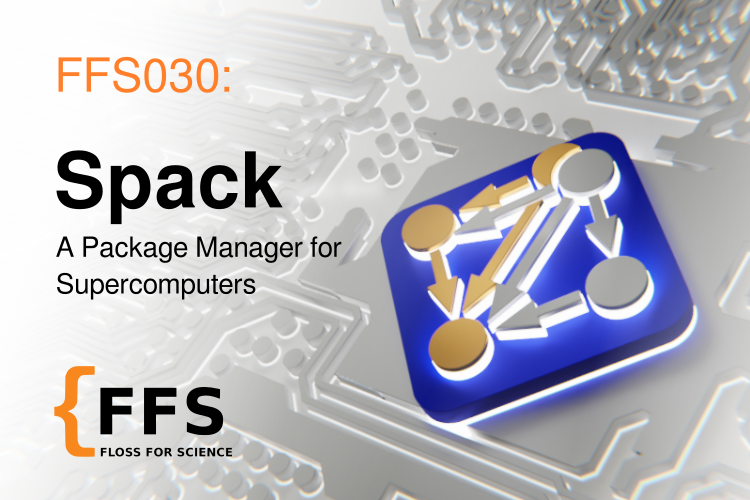
\includegraphics[width=0.5\linewidth]{FFS030_header.png}
    \hfill
    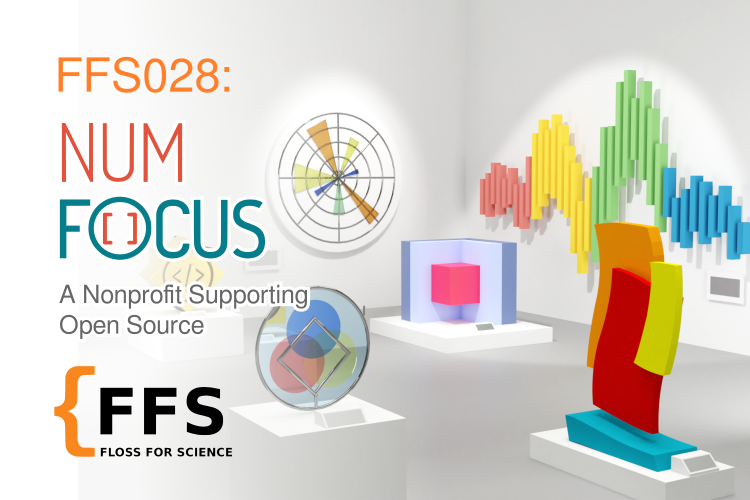
\includegraphics[width=0.5\linewidth]{FFS028_header.png}\\
    \vspace{0.5cm}
    
\includegraphics[width=0.5\linewidth]{FFS027_header.png}
    \hfill
    
\includegraphics[width=0.5\linewidth]{FFS019_header.png}
  \end{minipage}
\end{frame}

\begin{frame}{Open source software for production}

    \begin{itemize}
        \item Low-cost hardware is readily available
        \item The software components required for high quality audio production are available with open source licenses under Linux
        \item It is strongly recommended to record every participant on individual audio tracks to adjust their audio level separately
        \begin{itemize}
            \item The setup to record a podcast with all participants on a single track will be significantly easier to prepare and manage, but we chose to go with a multitrack setup for high audio quality
        \end{itemize}
    \end{itemize}
    
\end{frame}

\begin{frame}{Open source software for production}

    Hardware setup for local and remote podcast recording (\textasciitilde \$400 -- \$450):
    \begin{itemize}
        \item Behringer UMC404HD audio interface (\$180)
        \begin{itemize}
            \item Up to 4 local participants
            \item One Shure SM58 (\$99) for each local participant
        \end{itemize}
        \item Samson Q2U USB microphone for remote participants (\$70)
        \begin{itemize}
            \item It is possible to avoid the purchase of an audio interface if all participants are remote
        \end{itemize}
        \item Other class-compliant audio interfaces and microphones are available
        \item One computer serves as a central node for the remote and local recording
        \begin{itemize}
            \item General use computers are plenty sufficient
            \item Recording for FFS was performed on either a Thinkpad W530 or a Thinkpad X260
            \item The computer will need stable network connectivity
        \end{itemize}
        \item A multichannel headphone amplifier (\$35) is strongly suggested to give audio feedback for all local participants and improve their posture while recording
    \end{itemize}

\end{frame}

\begin{frame}{Open source software for production}

    General software
    \begin{itemize}
        \item Jitsi.meet
        \begin{itemize}
            \item VOIP software for remote participants
            \item The only requirement for the participants is a WebRTC compatible web browser
        \end{itemize}
        \item Chromium
        \begin{itemize}
            \item Separate Jitsi.meet instances on different tabs
            \item Firefox did not allow splitting the audio from different tabs into multiple channels \emoji{worried-face}
        \end{itemize}
        \item Linux
        \begin{itemize}
            \item All packages are available in Ubuntu from the main or third-party repositories
            \item Any Linux distribution can be made to work
            \item Ubuntu Studio is an easy all-in-one solution for beginners
            \item Real time or low latency kernel are suggested but not absolutely required for less demanding recording situations such as podcast recording
        \end{itemize}
    \end{itemize}

\end{frame}

\begin{frame}{Open source software for production}

    Audio software
    \begin{itemize}
        \item JACK (will eventualy be replaced by PipeWire for an easier setup)
        \begin{itemize}
            \item JACK Audio Connection Kit
            \item Linux low latency audio stack
            \item Allow special routing between different sources and sinks
            \item Need to be properly configured to create bridges to PulseAudio
        \end{itemize}
    \end{itemize}

\begin{columns}

    \begin{column}{0.4\linewidth}
        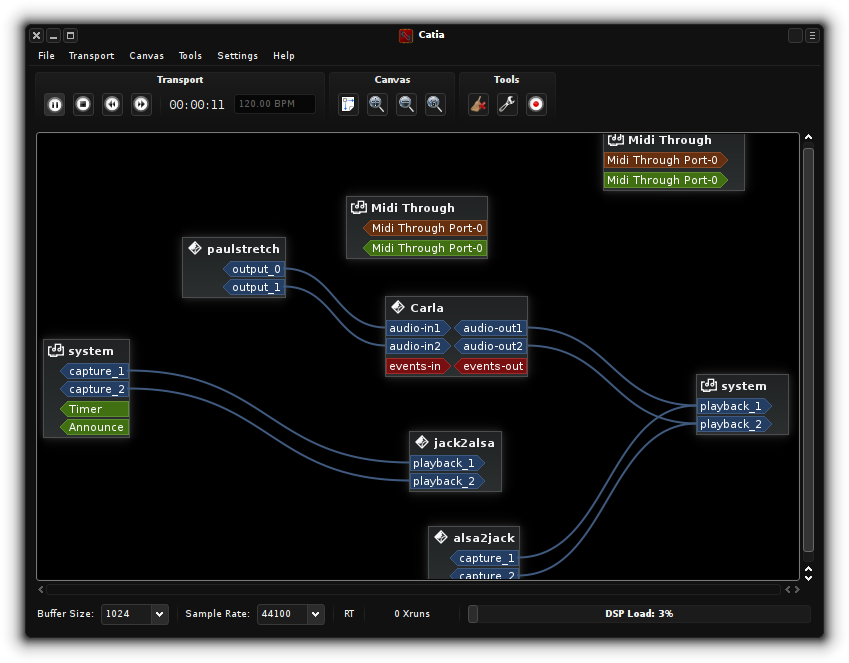
\includegraphics[width=\linewidth]{catia.png}
    \end{column}

    \begin{column}{0.6\linewidth}
        \begin{itemize}
            \item A JACK session manager and routing software (for graphical routing)
            \begin{itemize}
                \item Multiple combination/alternatives
                \item Cadence
                \item Ubuntu Studio Controls
                \item Qjackctl
                \item Catia
                \item Patchage
            \end{itemize}
        \end{itemize}
    \end{column}
    
    \end{columns}

\end{frame}

\begin{frame}{Open source software for production}

    Audio software

    \begin{columns}

    \begin{column}{0.4\linewidth}
        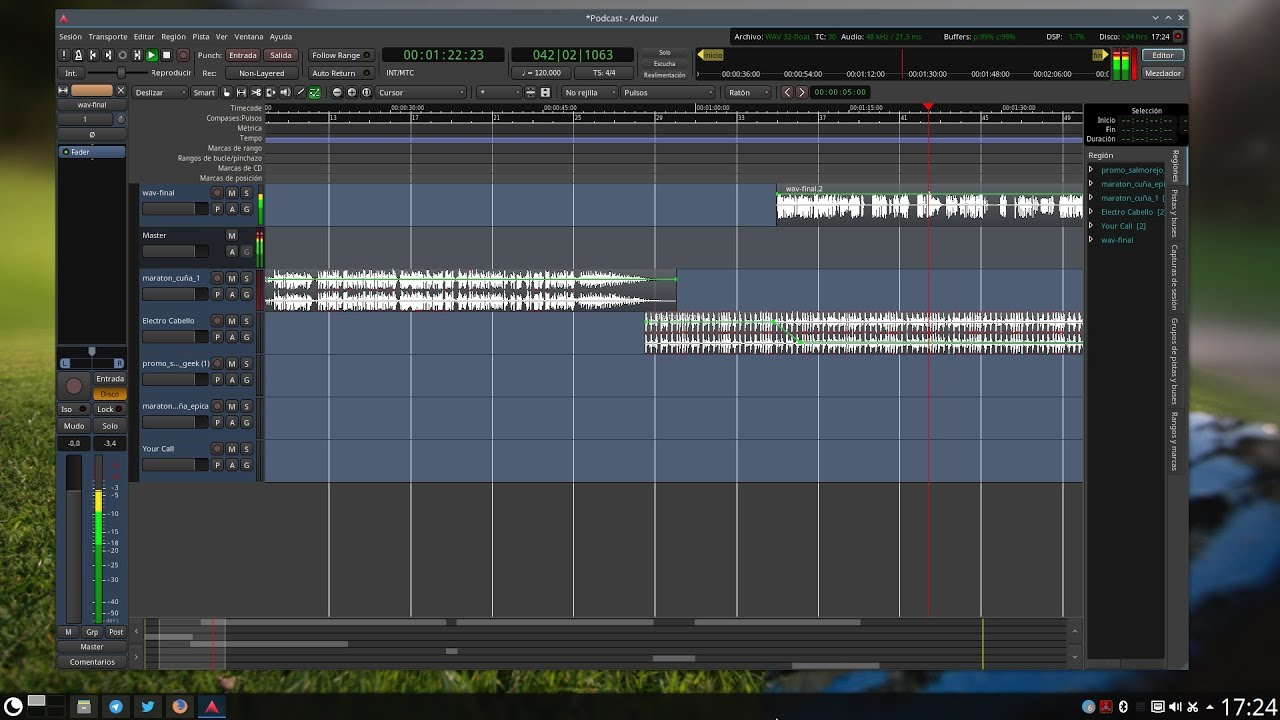
\includegraphics[width=\linewidth]{maxresdefault.jpg}
    \end{column}

    \begin{column}{0.6\linewidth}
        \begin{itemize}
            \item Ardour
            \begin{itemize}
                \item Multitrack audio recorder and editor
                \item Plugin host (denoise, gate, compressor, limiter, etc.)
            \end{itemize}
      
            \item CALF plugins
            \begin{itemize}
                \item Decent and easy to use audio plugins
                \item Gate, Compressor, Limiter...
            \end{itemize}
        \end{itemize}
    \end{column}
    
    \end{columns}

\vspace{6pt}

Other software and services
\begin{itemize}
    \item Media file hosting on Archive.org
    \item Website hosting on Github-pages
    \item Jeckyl static generated website
    \item Audio levelling with Auphonic online (non-free software)
\end{itemize}

\end{frame}


\begin{frame}{Lessons learned}

\begin{block}{Surprising}
    \begin{itemize}
        \item Was quite easy to find people willing to be interviewed,
        \item A professional graphic designer volunteered helping with the artwork
        \item Some episodes had over 600 listeners
    \end{itemize}
\end{block}

\begin{block}{Challenges}
    \begin{itemize}
        \item Was sometimes difficult to schedule interviews, \emph{e.g.}\ time zones, working hours.
        \item High quality audio is important, however, editing took much time out of David's resources.
        \item Funding is needed for editing, however, we want to avoid advertisement or sponsoring
    \end{itemize}
\end{block}
    
\end{frame}